\documentclass[twoside]{book}

% Packages required by doxygen
\usepackage{fixltx2e}
\usepackage{calc}
\usepackage{doxygen}
\usepackage[export]{adjustbox} % also loads graphicx
\usepackage{graphicx}
\usepackage[utf8]{inputenc}
\usepackage{makeidx}
\usepackage{multicol}
\usepackage{multirow}
\PassOptionsToPackage{warn}{textcomp}
\usepackage{textcomp}
\usepackage[nointegrals]{wasysym}
\usepackage[table]{xcolor}

% Font selection
\usepackage[T1]{fontenc}
\usepackage[scaled=.90]{helvet}
\usepackage{courier}
\usepackage{amssymb}
\usepackage{sectsty}
\renewcommand{\familydefault}{\sfdefault}
\allsectionsfont{%
  \fontseries{bc}\selectfont%
  \color{darkgray}%
}
\renewcommand{\DoxyLabelFont}{%
  \fontseries{bc}\selectfont%
  \color{darkgray}%
}
\newcommand{\+}{\discretionary{\mbox{\scriptsize$\hookleftarrow$}}{}{}}

% Page & text layout
\usepackage{geometry}
\geometry{%
  a4paper,%
  top=2.5cm,%
  bottom=2.5cm,%
  left=2.5cm,%
  right=2.5cm%
}
\tolerance=750
\hfuzz=15pt
\hbadness=750
\setlength{\emergencystretch}{15pt}
\setlength{\parindent}{0cm}
\setlength{\parskip}{3ex plus 2ex minus 2ex}
\makeatletter
\renewcommand{\paragraph}{%
  \@startsection{paragraph}{4}{0ex}{-1.0ex}{1.0ex}{%
    \normalfont\normalsize\bfseries\SS@parafont%
  }%
}
\renewcommand{\subparagraph}{%
  \@startsection{subparagraph}{5}{0ex}{-1.0ex}{1.0ex}{%
    \normalfont\normalsize\bfseries\SS@subparafont%
  }%
}
\makeatother

% Headers & footers
\usepackage{fancyhdr}
\pagestyle{fancyplain}
\fancyhead[LE]{\fancyplain{}{\bfseries\thepage}}
\fancyhead[CE]{\fancyplain{}{}}
\fancyhead[RE]{\fancyplain{}{\bfseries\leftmark}}
\fancyhead[LO]{\fancyplain{}{\bfseries\rightmark}}
\fancyhead[CO]{\fancyplain{}{}}
\fancyhead[RO]{\fancyplain{}{\bfseries\thepage}}
\fancyfoot[LE]{\fancyplain{}{}}
\fancyfoot[CE]{\fancyplain{}{}}
\fancyfoot[RE]{\fancyplain{}{\bfseries\scriptsize Generated by Doxygen }}
\fancyfoot[LO]{\fancyplain{}{\bfseries\scriptsize Generated by Doxygen }}
\fancyfoot[CO]{\fancyplain{}{}}
\fancyfoot[RO]{\fancyplain{}{}}
\renewcommand{\footrulewidth}{0.4pt}
\renewcommand{\chaptermark}[1]{%
  \markboth{#1}{}%
}
\renewcommand{\sectionmark}[1]{%
  \markright{\thesection\ #1}%
}

% Indices & bibliography
\usepackage{natbib}
\usepackage[titles]{tocloft}
\setcounter{tocdepth}{3}
\setcounter{secnumdepth}{5}
\makeindex

% Hyperlinks (required, but should be loaded last)
\usepackage{ifpdf}
\ifpdf
  \usepackage[pdftex,pagebackref=true]{hyperref}
\else
  \usepackage[ps2pdf,pagebackref=true]{hyperref}
\fi
\hypersetup{%
  colorlinks=true,%
  linkcolor=blue,%
  citecolor=blue,%
  unicode%
}

% Custom commands
\newcommand{\clearemptydoublepage}{%
  \newpage{\pagestyle{empty}\cleardoublepage}%
}

\usepackage{caption}
\captionsetup{labelsep=space,justification=centering,font={bf},singlelinecheck=off,skip=4pt,position=top}

%===== C O N T E N T S =====

\begin{document}

% Titlepage & ToC
\hypersetup{pageanchor=false,
             bookmarksnumbered=true,
             pdfencoding=unicode
            }
\pagenumbering{roman}
\begin{titlepage}
\vspace*{7cm}
\begin{center}%
{\Large My Project }\\
\vspace*{1cm}
{\large Generated by Doxygen 1.8.11}\\
\end{center}
\end{titlepage}
\clearemptydoublepage
\tableofcontents
\clearemptydoublepage
\pagenumbering{arabic}
\hypersetup{pageanchor=true}

%--- Begin generated contents ---
\chapter{\+\_\+\+Footer}
\label{md_packages_EWSoftware.SHFB.2016.4.9.0_tools_PresentationStyles_Markdown_MarkdownContent__Footer}
\hypertarget{md_packages_EWSoftware.SHFB.2016.4.9.0_tools_PresentationStyles_Markdown_MarkdownContent__Footer}{}
\{\}

\{\} \{\} Send comments on this topic to \mbox{[}\{\}\mbox{]}(mailto\+:\{\}?Subject=\{\}) 
\chapter{Namespace Index}
\section{Namespace List}
Here is a list of all documented namespaces with brief descriptions\+:\begin{DoxyCompactList}
\item\contentsline{section}{\hyperlink{namespace__1920_parser}{\+\_\+1920\+Parser} }{\pageref{namespace__1920_parser}}{}
\item\contentsline{section}{\hyperlink{namespace__1920_parser_1_1_properties}{\+\_\+1920\+Parser.\+Properties} }{\pageref{namespace__1920_parser_1_1_properties}}{}
\end{DoxyCompactList}

\chapter{Hierarchical Index}
\section{Class Hierarchy}
This inheritance list is sorted roughly, but not completely, alphabetically\+:\begin{DoxyCompactList}
\item \contentsline{section}{\+\_\+1920\+Parser.\+Abstract\+Node}{\pageref{class__1920_parser_1_1_abstract_node}}{}
\begin{DoxyCompactList}
\item \contentsline{section}{\+\_\+1920\+Parser.\+Group\+Node}{\pageref{class__1920_parser_1_1_group_node}}{}
\item \contentsline{section}{\+\_\+1920\+Parser.\+Value\+Node}{\pageref{class__1920_parser_1_1_value_node}}{}
\end{DoxyCompactList}
\item Form\begin{DoxyCompactList}
\item \contentsline{section}{\+\_\+1920\+Parser.\+\_\+1920\+Parser\+Form}{\pageref{class__1920_parser_1_1__1920_parser_form}}{}
\item \contentsline{section}{\+\_\+1920\+Parser.\+Save\+Schema\+Form}{\pageref{class__1920_parser_1_1_save_schema_form}}{}
\end{DoxyCompactList}
\item \contentsline{section}{\+\_\+1920\+Parser.\+Schema}{\pageref{class__1920_parser_1_1_schema}}{}
\item \contentsline{section}{schemas}{\pageref{classschemas}}{}
\item \contentsline{section}{schemas\+Schema}{\pageref{classschemas_schema}}{}
\item \contentsline{section}{schemas\+Schema\+Identifier}{\pageref{classschemas_schema_identifier}}{}
\end{DoxyCompactList}

\chapter{Class Index}
\section{Class List}
Here are the classes, structs, unions and interfaces with brief descriptions\+:\begin{DoxyCompactList}
\item\contentsline{section}{\hyperlink{class__1920_parser_1_1__1920_parser_form}{\+\_\+1920\+Parser.\+\_\+1920\+Parser\+Form} \\*asdfjkalaega sadfjkl asdfhsa sadfha /summary$>$ }{\pageref{class__1920_parser_1_1__1920_parser_form}}{}
\item\contentsline{section}{\hyperlink{class__1920_parser_1_1_abstract_node}{\+\_\+1920\+Parser.\+Abstract\+Node} \\*}{\pageref{class__1920_parser_1_1_abstract_node}}{}
\item\contentsline{section}{\hyperlink{class_activity_designer_library1_1_1_activity_designer1}{Activity\+Designer\+Library1.\+Activity\+Designer1} \\*\hyperlink{class_activity_designer_library1_1_1_activity_designer1}{Activity\+Designer1} }{\pageref{class_activity_designer_library1_1_1_activity_designer1}}{}
\item\contentsline{section}{\hyperlink{class__1920_parser_1_1_group_node}{\+\_\+1920\+Parser.\+Group\+Node} \\*\hyperlink{class__1920_parser_1_1_group_node}{Group\+Node} represents an internal node. }{\pageref{class__1920_parser_1_1_group_node}}{}
\item\contentsline{section}{\hyperlink{class__1920_parser_test_1_1_group_node_test}{\+\_\+1920\+Parser\+Test.\+Group\+Node\+Test} \\*This is a test class for \hyperlink{class__1920_parser_test_1_1_group_node_test}{Group\+Node\+Test} and is intended to contain all \hyperlink{class__1920_parser_test_1_1_group_node_test}{Group\+Node\+Test} Unit Tests /summary$>$ }{\pageref{class__1920_parser_test_1_1_group_node_test}}{}
\item\contentsline{section}{\hyperlink{class_ranking}{Ranking} }{\pageref{class_ranking}}{}
\item\contentsline{section}{\hyperlink{class__1920_parser_1_1_save_schema_form}{\+\_\+1920\+Parser.\+Save\+Schema\+Form} }{\pageref{class__1920_parser_1_1_save_schema_form}}{}
\item\contentsline{section}{\hyperlink{class__1920_parser_1_1_schema}{\+\_\+1920\+Parser.\+Schema} }{\pageref{class__1920_parser_1_1_schema}}{}
\item\contentsline{section}{\hyperlink{classschemas}{schemas} \\*}{\pageref{classschemas}}{}
\item\contentsline{section}{\hyperlink{classschemas_schema}{schemas\+Schema} \\*}{\pageref{classschemas_schema}}{}
\item\contentsline{section}{\hyperlink{classschemas_schema_identifier}{schemas\+Schema\+Identifier} \\*}{\pageref{classschemas_schema_identifier}}{}
\item\contentsline{section}{\hyperlink{class__1920_parser_test_1_1_schema_test}{\+\_\+1920\+Parser\+Test.\+Schema\+Test} \\*This is a test class for \hyperlink{class__1920_parser_test_1_1_schema_test}{Schema\+Test} and is intended to contain all \hyperlink{class__1920_parser_test_1_1_schema_test}{Schema\+Test} Unit Tests /summary$>$ }{\pageref{class__1920_parser_test_1_1_schema_test}}{}
\item\contentsline{section}{\hyperlink{class__1920_parser_1_1_value_node}{\+\_\+1920\+Parser.\+Value\+Node} }{\pageref{class__1920_parser_1_1_value_node}}{}
\item\contentsline{section}{\hyperlink{class__1920_parser_test_1_1_value_node_test}{\+\_\+1920\+Parser\+Test.\+Value\+Node\+Test} \\*This is a test class for \hyperlink{class__1920_parser_test_1_1_value_node_test}{Value\+Node\+Test} and is intended to contain all \hyperlink{class__1920_parser_test_1_1_value_node_test}{Value\+Node\+Test} Unit Tests /summary$>$ }{\pageref{class__1920_parser_test_1_1_value_node_test}}{}
\end{DoxyCompactList}

\chapter{Namespace Documentation}
\hypertarget{namespace__1920_parser}{}\section{\+\_\+1920\+Parser Namespace Reference}
\label{namespace__1920_parser}\index{\+\_\+1920\+Parser@{\+\_\+1920\+Parser}}
\subsection*{Classes}
\begin{DoxyCompactItemize}
\item 
class \hyperlink{class__1920_parser_1_1__1920_parser_form}{\+\_\+1920\+Parser\+Form}
\begin{DoxyCompactList}\small\item\em asdfjkalaega sadfjkl asdfhsa sadfha /summary$>$ \end{DoxyCompactList}\item 
class \hyperlink{class__1920_parser_1_1_abstract_node}{Abstract\+Node}
\item 
class \hyperlink{class__1920_parser_1_1_group_node}{Group\+Node}
\begin{DoxyCompactList}\small\item\em testclasdfjkl \end{DoxyCompactList}\item 
class \hyperlink{class__1920_parser_1_1_save_schema_form}{Save\+Schema\+Form}
\item 
class \hyperlink{class__1920_parser_1_1_schema}{Schema}
\item 
class \hyperlink{class__1920_parser_1_1_value_node}{Value\+Node}
\end{DoxyCompactItemize}

\hypertarget{namespace__1920_parser_1_1_properties}{}\section{\+\_\+1920\+Parser.\+Properties Namespace Reference}
\label{namespace__1920_parser_1_1_properties}\index{\+\_\+1920\+Parser.\+Properties@{\+\_\+1920\+Parser.\+Properties}}
\subsection*{Classes}
\begin{DoxyCompactItemize}
\item 
class {\bfseries Resources}
\begin{DoxyCompactList}\small\item\em A strongly-\/typed resource class, for looking up localized strings, etc. \end{DoxyCompactList}\item 
class {\bfseries Settings}
\end{DoxyCompactItemize}

\hypertarget{namespace__1920_parser_test}{}\section{\+\_\+1920\+Parser\+Test Namespace Reference}
\label{namespace__1920_parser_test}\index{\+\_\+1920\+Parser\+Test@{\+\_\+1920\+Parser\+Test}}
\subsection*{Classes}
\begin{DoxyCompactItemize}
\item 
class \hyperlink{class__1920_parser_test_1_1_group_node_test}{Group\+Node\+Test}
\begin{DoxyCompactList}\small\item\em This is a test class for \hyperlink{class__1920_parser_test_1_1_group_node_test}{Group\+Node\+Test} and is intended to contain all \hyperlink{class__1920_parser_test_1_1_group_node_test}{Group\+Node\+Test} Unit Tests /summary$>$ \end{DoxyCompactList}\item 
class \hyperlink{class__1920_parser_test_1_1_schema_test}{Schema\+Test}
\begin{DoxyCompactList}\small\item\em This is a test class for \hyperlink{class__1920_parser_test_1_1_schema_test}{Schema\+Test} and is intended to contain all \hyperlink{class__1920_parser_test_1_1_schema_test}{Schema\+Test} Unit Tests /summary$>$ \end{DoxyCompactList}\item 
class \hyperlink{class__1920_parser_test_1_1_value_node_test}{Value\+Node\+Test}
\begin{DoxyCompactList}\small\item\em This is a test class for \hyperlink{class__1920_parser_test_1_1_value_node_test}{Value\+Node\+Test} and is intended to contain all \hyperlink{class__1920_parser_test_1_1_value_node_test}{Value\+Node\+Test} Unit Tests /summary$>$ \end{DoxyCompactList}\end{DoxyCompactItemize}

\hypertarget{namespace_activity_designer_library1}{}\section{Activity\+Designer\+Library1 Namespace Reference}
\label{namespace_activity_designer_library1}\index{Activity\+Designer\+Library1@{Activity\+Designer\+Library1}}
\subsection*{Namespaces}
\begin{DoxyCompactItemize}
\end{DoxyCompactItemize}
\subsection*{Classes}
\begin{DoxyCompactItemize}
\item 
class \hyperlink{class_activity_designer_library1_1_1_activity_designer1}{Activity\+Designer1}
\begin{DoxyCompactList}\small\item\em \hyperlink{class_activity_designer_library1_1_1_activity_designer1}{Activity\+Designer1} \end{DoxyCompactList}\end{DoxyCompactItemize}

\hypertarget{namespace_activity_designer_library1_1_1_properties}{}\section{Activity\+Designer\+Library1.\+Properties Namespace Reference}
\label{namespace_activity_designer_library1_1_1_properties}\index{Activity\+Designer\+Library1.\+Properties@{Activity\+Designer\+Library1.\+Properties}}
\subsection*{Classes}
\begin{DoxyCompactItemize}
\item 
class {\bfseries Resources}
\begin{DoxyCompactList}\small\item\em A strongly-\/typed resource class, for looking up localized strings, etc. \end{DoxyCompactList}\item 
class {\bfseries Settings}
\end{DoxyCompactItemize}

\chapter{Class Documentation}
\hypertarget{class__1920_parser_1_1__1920_parser_form}{}\section{\+\_\+1920\+Parser.\+\_\+1920\+Parser\+Form Class Reference}
\label{class__1920_parser_1_1__1920_parser_form}\index{\+\_\+1920\+Parser.\+\_\+1920\+Parser\+Form@{\+\_\+1920\+Parser.\+\_\+1920\+Parser\+Form}}


asdfjkalaega sadfjkl asdfhsa sadfha /summary$>$  


Inheritance diagram for \+\_\+1920\+Parser.\+\_\+1920\+Parser\+Form\+:\begin{figure}[H]
\begin{center}
\leavevmode
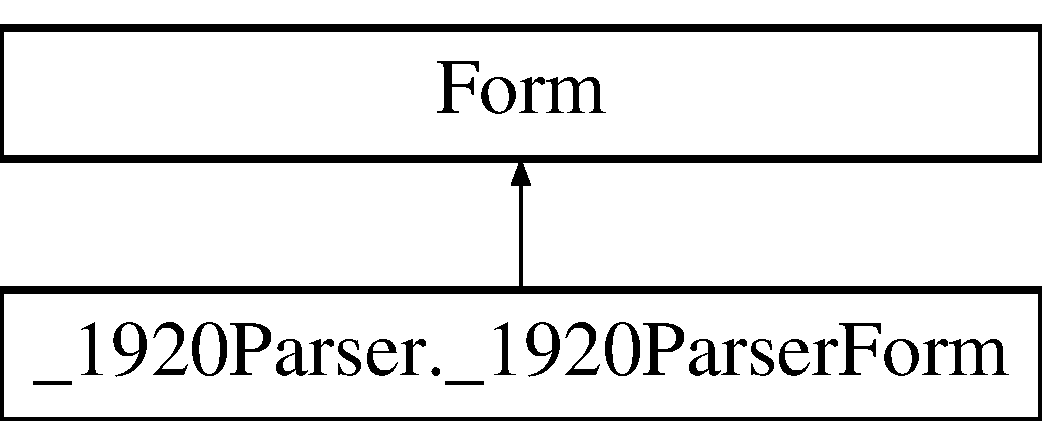
\includegraphics[height=2.000000cm]{class__1920_parser_1_1__1920_parser_form}
\end{center}
\end{figure}
\subsection*{Public Member Functions}
\begin{DoxyCompactItemize}
\item 
\hyperlink{class__1920_parser_1_1__1920_parser_form_ad4ad99c74a78589f16c5a75d7f0eda22}{\+\_\+1920\+Parser\+Form} ()
\end{DoxyCompactItemize}
\subsection*{Protected Member Functions}
\begin{DoxyCompactItemize}
\item 
override void \hyperlink{class__1920_parser_1_1__1920_parser_form_a834ea0eefb07ff1fdd7afea7a20834fa}{Dispose} (bool disposing)
\begin{DoxyCompactList}\small\item\em Clean up any resources being used. \end{DoxyCompactList}\end{DoxyCompactItemize}


\subsection{Detailed Description}
asdfjkalaega sadfjkl asdfhsa sadfha /summary$>$ 

\subsection{Constructor \& Destructor Documentation}
\index{\+\_\+1920\+Parser\+::\+\_\+1920\+Parser\+Form@{\+\_\+1920\+Parser\+::\+\_\+1920\+Parser\+Form}!\+\_\+1920\+Parser\+Form@{\+\_\+1920\+Parser\+Form}}
\index{\+\_\+1920\+Parser\+Form@{\+\_\+1920\+Parser\+Form}!\+\_\+1920\+Parser\+::\+\_\+1920\+Parser\+Form@{\+\_\+1920\+Parser\+::\+\_\+1920\+Parser\+Form}}
\subsubsection[{\texorpdfstring{\+\_\+1920\+Parser\+Form()}{_1920ParserForm()}}]{\setlength{\rightskip}{0pt plus 5cm}\+\_\+1920\+Parser.\+\_\+1920\+Parser\+Form.\+\_\+1920\+Parser\+Form (
\begin{DoxyParamCaption}
{}
\end{DoxyParamCaption}
)}\hypertarget{class__1920_parser_1_1__1920_parser_form_ad4ad99c74a78589f16c5a75d7f0eda22}{}\label{class__1920_parser_1_1__1920_parser_form_ad4ad99c74a78589f16c5a75d7f0eda22}


\subsection{Member Function Documentation}
\index{\+\_\+1920\+Parser\+::\+\_\+1920\+Parser\+Form@{\+\_\+1920\+Parser\+::\+\_\+1920\+Parser\+Form}!Dispose@{Dispose}}
\index{Dispose@{Dispose}!\+\_\+1920\+Parser\+::\+\_\+1920\+Parser\+Form@{\+\_\+1920\+Parser\+::\+\_\+1920\+Parser\+Form}}
\subsubsection[{\texorpdfstring{Dispose(bool disposing)}{Dispose(bool disposing)}}]{\setlength{\rightskip}{0pt plus 5cm}override void \+\_\+1920\+Parser.\+\_\+1920\+Parser\+Form.\+Dispose (
\begin{DoxyParamCaption}
\item[{bool}]{disposing}
\end{DoxyParamCaption}
)\hspace{0.3cm}{\ttfamily [protected]}}\hypertarget{class__1920_parser_1_1__1920_parser_form_a834ea0eefb07ff1fdd7afea7a20834fa}{}\label{class__1920_parser_1_1__1920_parser_form_a834ea0eefb07ff1fdd7afea7a20834fa}


Clean up any resources being used. 


\begin{DoxyParams}{Parameters}
{\em disposing} & true if managed resources should be disposed; otherwise, false.\\
\hline
\end{DoxyParams}


The documentation for this class was generated from the following files\+:\begin{DoxyCompactItemize}
\item 
\hyperlink{1920_parser_form_8cs}{1920\+Parser\+Form.\+cs}\item 
\hyperlink{1920_parser_form_8_designer_8cs}{1920\+Parser\+Form.\+Designer.\+cs}\end{DoxyCompactItemize}

\hypertarget{class__1920_parser_1_1_abstract_node}{}\section{\+\_\+1920\+Parser.\+Abstract\+Node Class Reference}
\label{class__1920_parser_1_1_abstract_node}\index{\+\_\+1920\+Parser.\+Abstract\+Node@{\+\_\+1920\+Parser.\+Abstract\+Node}}


 


Inheritance diagram for \+\_\+1920\+Parser.\+Abstract\+Node\+:\begin{figure}[H]
\begin{center}
\leavevmode
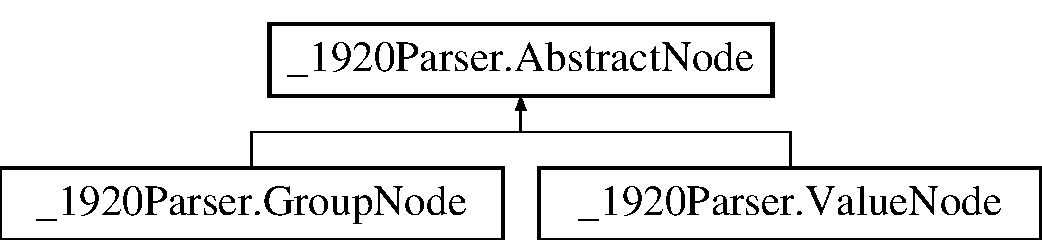
\includegraphics[height=2.000000cm]{class__1920_parser_1_1_abstract_node}
\end{center}
\end{figure}
\subsection*{Public Member Functions}
\begin{DoxyCompactItemize}
\item 
\hyperlink{class__1920_parser_1_1_abstract_node_aebc3c9efb2855add3285f717edd5ca86}{Abstract\+Node} (bool redefines, int level, string var\+Name, int repeat\+Count, int repeat\+Index, string comment)
\item 
abstract \hyperlink{class__1920_parser_1_1_abstract_node}{Abstract\+Node} \hyperlink{class__1920_parser_1_1_abstract_node_a636ae975a7e037fb31c4d4341e222c1b}{Create\+Copy\+With\+Index} (int index)
\item 
abstract int \hyperlink{class__1920_parser_1_1_abstract_node_a457498d3ec29d4c2af707aad2cf3bfc9}{Assign\+Value} (string data)
\item 
abstract string \hyperlink{class__1920_parser_1_1_abstract_node_ae41877e0bad1b9ed1e4b5ae8c01bca60}{To\+String} (int tab\+Count)
\item 
override string \hyperlink{class__1920_parser_1_1_abstract_node_a2fef1588cfaa3d7979c8fd3af77d08d3}{To\+String} ()
\item 
abstract void \hyperlink{class__1920_parser_1_1_abstract_node_af6241531937bb83d55aea81268b97f0b}{Add\+Child} (\hyperlink{class__1920_parser_1_1_abstract_node}{Abstract\+Node} child)
\end{DoxyCompactItemize}
\subsection*{Properties}
\begin{DoxyCompactItemize}
\item 
bool \hyperlink{class__1920_parser_1_1_abstract_node_a66fd8845fa232c78f396f15467e17458}{Redefines}\hspace{0.3cm}{\ttfamily  \mbox{[}get, protected set\mbox{]}}
\begin{DoxyCompactList}\small\item\em Gets or sets a value indicating whether this \hyperlink{class__1920_parser_1_1_abstract_node}{Abstract\+Node} is redefines. \end{DoxyCompactList}\item 
int \hyperlink{class__1920_parser_1_1_abstract_node_a08c3c1dccbd57a5ddf4c6f2144223dc6}{Level}\hspace{0.3cm}{\ttfamily  \mbox{[}get, protected set\mbox{]}}
\begin{DoxyCompactList}\small\item\em Gets or sets the level. \end{DoxyCompactList}\item 
string \hyperlink{class__1920_parser_1_1_abstract_node_ae4a8076d5cf940c9fa0b1a7fecdd4a6a}{Var\+Name}\hspace{0.3cm}{\ttfamily  \mbox{[}get, protected set\mbox{]}}
\begin{DoxyCompactList}\small\item\em Gets or sets the name of the variable. \end{DoxyCompactList}\item 
int \hyperlink{class__1920_parser_1_1_abstract_node_a68d196e888509c7a603ea9f89124cd11}{Repeat\+Count}\hspace{0.3cm}{\ttfamily  \mbox{[}get, protected set\mbox{]}}
\item 
int \hyperlink{class__1920_parser_1_1_abstract_node_a727fdfa1025e8c672a28c60bef03d9b9}{Repeat\+Index}\hspace{0.3cm}{\ttfamily  \mbox{[}get, protected set\mbox{]}}
\item 
string \hyperlink{class__1920_parser_1_1_abstract_node_aff4df7a21266685abdac7a455a0f7ac8}{Comment}\hspace{0.3cm}{\ttfamily  \mbox{[}get, protected set\mbox{]}}
\end{DoxyCompactItemize}


\subsection{Detailed Description}




\subsection{Constructor \& Destructor Documentation}
\index{\+\_\+1920\+Parser\+::\+Abstract\+Node@{\+\_\+1920\+Parser\+::\+Abstract\+Node}!Abstract\+Node@{Abstract\+Node}}
\index{Abstract\+Node@{Abstract\+Node}!\+\_\+1920\+Parser\+::\+Abstract\+Node@{\+\_\+1920\+Parser\+::\+Abstract\+Node}}
\subsubsection[{\texorpdfstring{Abstract\+Node(bool redefines, int level, string var\+Name, int repeat\+Count, int repeat\+Index, string comment)}{AbstractNode(bool redefines, int level, string varName, int repeatCount, int repeatIndex, string comment)}}]{\setlength{\rightskip}{0pt plus 5cm}\+\_\+1920\+Parser.\+Abstract\+Node.\+Abstract\+Node (
\begin{DoxyParamCaption}
\item[{bool}]{redefines, }
\item[{int}]{level, }
\item[{string}]{var\+Name, }
\item[{int}]{repeat\+Count, }
\item[{int}]{repeat\+Index, }
\item[{string}]{comment}
\end{DoxyParamCaption}
)}\hypertarget{class__1920_parser_1_1_abstract_node_aebc3c9efb2855add3285f717edd5ca86}{}\label{class__1920_parser_1_1_abstract_node_aebc3c9efb2855add3285f717edd5ca86}


\subsection{Member Function Documentation}
\index{\+\_\+1920\+Parser\+::\+Abstract\+Node@{\+\_\+1920\+Parser\+::\+Abstract\+Node}!Add\+Child@{Add\+Child}}
\index{Add\+Child@{Add\+Child}!\+\_\+1920\+Parser\+::\+Abstract\+Node@{\+\_\+1920\+Parser\+::\+Abstract\+Node}}
\subsubsection[{\texorpdfstring{Add\+Child(\+Abstract\+Node child)}{AddChild(AbstractNode child)}}]{\setlength{\rightskip}{0pt plus 5cm}abstract void \+\_\+1920\+Parser.\+Abstract\+Node.\+Add\+Child (
\begin{DoxyParamCaption}
\item[{{\bf Abstract\+Node}}]{child}
\end{DoxyParamCaption}
)\hspace{0.3cm}{\ttfamily [pure virtual]}}\hypertarget{class__1920_parser_1_1_abstract_node_af6241531937bb83d55aea81268b97f0b}{}\label{class__1920_parser_1_1_abstract_node_af6241531937bb83d55aea81268b97f0b}


Implemented in \hyperlink{class__1920_parser_1_1_group_node_a037839ecea0ec7326c6a49e0793bd6c8}{\+\_\+1920\+Parser.\+Group\+Node}, and \hyperlink{class__1920_parser_1_1_value_node_a035c2fb0a7af286a4718e7215b2925a1}{\+\_\+1920\+Parser.\+Value\+Node}.

\index{\+\_\+1920\+Parser\+::\+Abstract\+Node@{\+\_\+1920\+Parser\+::\+Abstract\+Node}!Assign\+Value@{Assign\+Value}}
\index{Assign\+Value@{Assign\+Value}!\+\_\+1920\+Parser\+::\+Abstract\+Node@{\+\_\+1920\+Parser\+::\+Abstract\+Node}}
\subsubsection[{\texorpdfstring{Assign\+Value(string data)}{AssignValue(string data)}}]{\setlength{\rightskip}{0pt plus 5cm}abstract int \+\_\+1920\+Parser.\+Abstract\+Node.\+Assign\+Value (
\begin{DoxyParamCaption}
\item[{string}]{data}
\end{DoxyParamCaption}
)\hspace{0.3cm}{\ttfamily [pure virtual]}}\hypertarget{class__1920_parser_1_1_abstract_node_a457498d3ec29d4c2af707aad2cf3bfc9}{}\label{class__1920_parser_1_1_abstract_node_a457498d3ec29d4c2af707aad2cf3bfc9}


Implemented in \hyperlink{class__1920_parser_1_1_value_node_a21bed203f8124c630e8b804ebcd7b728}{\+\_\+1920\+Parser.\+Value\+Node}, and \hyperlink{class__1920_parser_1_1_group_node_a27b61720154a26499149966cf22de811}{\+\_\+1920\+Parser.\+Group\+Node}.

\index{\+\_\+1920\+Parser\+::\+Abstract\+Node@{\+\_\+1920\+Parser\+::\+Abstract\+Node}!Create\+Copy\+With\+Index@{Create\+Copy\+With\+Index}}
\index{Create\+Copy\+With\+Index@{Create\+Copy\+With\+Index}!\+\_\+1920\+Parser\+::\+Abstract\+Node@{\+\_\+1920\+Parser\+::\+Abstract\+Node}}
\subsubsection[{\texorpdfstring{Create\+Copy\+With\+Index(int index)}{CreateCopyWithIndex(int index)}}]{\setlength{\rightskip}{0pt plus 5cm}abstract {\bf Abstract\+Node} \+\_\+1920\+Parser.\+Abstract\+Node.\+Create\+Copy\+With\+Index (
\begin{DoxyParamCaption}
\item[{int}]{index}
\end{DoxyParamCaption}
)\hspace{0.3cm}{\ttfamily [pure virtual]}}\hypertarget{class__1920_parser_1_1_abstract_node_a636ae975a7e037fb31c4d4341e222c1b}{}\label{class__1920_parser_1_1_abstract_node_a636ae975a7e037fb31c4d4341e222c1b}


Implemented in \hyperlink{class__1920_parser_1_1_group_node_ab01b00a2bbbef1d565e5ef3e951c4ed6}{\+\_\+1920\+Parser.\+Group\+Node}, and \hyperlink{class__1920_parser_1_1_value_node_a9419a8beace8e6eda482fc3a403daf4b}{\+\_\+1920\+Parser.\+Value\+Node}.

\index{\+\_\+1920\+Parser\+::\+Abstract\+Node@{\+\_\+1920\+Parser\+::\+Abstract\+Node}!To\+String@{To\+String}}
\index{To\+String@{To\+String}!\+\_\+1920\+Parser\+::\+Abstract\+Node@{\+\_\+1920\+Parser\+::\+Abstract\+Node}}
\subsubsection[{\texorpdfstring{To\+String(int tab\+Count)}{ToString(int tabCount)}}]{\setlength{\rightskip}{0pt plus 5cm}abstract string \+\_\+1920\+Parser.\+Abstract\+Node.\+To\+String (
\begin{DoxyParamCaption}
\item[{int}]{tab\+Count}
\end{DoxyParamCaption}
)\hspace{0.3cm}{\ttfamily [pure virtual]}}\hypertarget{class__1920_parser_1_1_abstract_node_ae41877e0bad1b9ed1e4b5ae8c01bca60}{}\label{class__1920_parser_1_1_abstract_node_ae41877e0bad1b9ed1e4b5ae8c01bca60}


Implemented in \hyperlink{class__1920_parser_1_1_group_node_a9d5c05eabdd12c9c4ca306cc369d8523}{\+\_\+1920\+Parser.\+Group\+Node}, and \hyperlink{class__1920_parser_1_1_value_node_ae2b512cbab33936e1b02d7a7acf3b4bd}{\+\_\+1920\+Parser.\+Value\+Node}.

\index{\+\_\+1920\+Parser\+::\+Abstract\+Node@{\+\_\+1920\+Parser\+::\+Abstract\+Node}!To\+String@{To\+String}}
\index{To\+String@{To\+String}!\+\_\+1920\+Parser\+::\+Abstract\+Node@{\+\_\+1920\+Parser\+::\+Abstract\+Node}}
\subsubsection[{\texorpdfstring{To\+String()}{ToString()}}]{\setlength{\rightskip}{0pt plus 5cm}override string \+\_\+1920\+Parser.\+Abstract\+Node.\+To\+String (
\begin{DoxyParamCaption}
{}
\end{DoxyParamCaption}
)}\hypertarget{class__1920_parser_1_1_abstract_node_a2fef1588cfaa3d7979c8fd3af77d08d3}{}\label{class__1920_parser_1_1_abstract_node_a2fef1588cfaa3d7979c8fd3af77d08d3}


\subsection{Property Documentation}
\index{\+\_\+1920\+Parser\+::\+Abstract\+Node@{\+\_\+1920\+Parser\+::\+Abstract\+Node}!Comment@{Comment}}
\index{Comment@{Comment}!\+\_\+1920\+Parser\+::\+Abstract\+Node@{\+\_\+1920\+Parser\+::\+Abstract\+Node}}
\subsubsection[{\texorpdfstring{Comment}{Comment}}]{\setlength{\rightskip}{0pt plus 5cm}string \+\_\+1920\+Parser.\+Abstract\+Node.\+Comment\hspace{0.3cm}{\ttfamily [get]}, {\ttfamily [protected set]}}\hypertarget{class__1920_parser_1_1_abstract_node_aff4df7a21266685abdac7a455a0f7ac8}{}\label{class__1920_parser_1_1_abstract_node_aff4df7a21266685abdac7a455a0f7ac8}
\index{\+\_\+1920\+Parser\+::\+Abstract\+Node@{\+\_\+1920\+Parser\+::\+Abstract\+Node}!Level@{Level}}
\index{Level@{Level}!\+\_\+1920\+Parser\+::\+Abstract\+Node@{\+\_\+1920\+Parser\+::\+Abstract\+Node}}
\subsubsection[{\texorpdfstring{Level}{Level}}]{\setlength{\rightskip}{0pt plus 5cm}int \+\_\+1920\+Parser.\+Abstract\+Node.\+Level\hspace{0.3cm}{\ttfamily [get]}, {\ttfamily [protected set]}}\hypertarget{class__1920_parser_1_1_abstract_node_a08c3c1dccbd57a5ddf4c6f2144223dc6}{}\label{class__1920_parser_1_1_abstract_node_a08c3c1dccbd57a5ddf4c6f2144223dc6}


Gets or sets the level. 

The level. \index{\+\_\+1920\+Parser\+::\+Abstract\+Node@{\+\_\+1920\+Parser\+::\+Abstract\+Node}!Redefines@{Redefines}}
\index{Redefines@{Redefines}!\+\_\+1920\+Parser\+::\+Abstract\+Node@{\+\_\+1920\+Parser\+::\+Abstract\+Node}}
\subsubsection[{\texorpdfstring{Redefines}{Redefines}}]{\setlength{\rightskip}{0pt plus 5cm}bool \+\_\+1920\+Parser.\+Abstract\+Node.\+Redefines\hspace{0.3cm}{\ttfamily [get]}, {\ttfamily [protected set]}}\hypertarget{class__1920_parser_1_1_abstract_node_a66fd8845fa232c78f396f15467e17458}{}\label{class__1920_parser_1_1_abstract_node_a66fd8845fa232c78f396f15467e17458}


Gets or sets a value indicating whether this \hyperlink{class__1920_parser_1_1_abstract_node}{Abstract\+Node} is redefines. 

{\ttfamily true} if redefines; otherwise, {\ttfamily false}. \index{\+\_\+1920\+Parser\+::\+Abstract\+Node@{\+\_\+1920\+Parser\+::\+Abstract\+Node}!Repeat\+Count@{Repeat\+Count}}
\index{Repeat\+Count@{Repeat\+Count}!\+\_\+1920\+Parser\+::\+Abstract\+Node@{\+\_\+1920\+Parser\+::\+Abstract\+Node}}
\subsubsection[{\texorpdfstring{Repeat\+Count}{RepeatCount}}]{\setlength{\rightskip}{0pt plus 5cm}int \+\_\+1920\+Parser.\+Abstract\+Node.\+Repeat\+Count\hspace{0.3cm}{\ttfamily [get]}, {\ttfamily [protected set]}}\hypertarget{class__1920_parser_1_1_abstract_node_a68d196e888509c7a603ea9f89124cd11}{}\label{class__1920_parser_1_1_abstract_node_a68d196e888509c7a603ea9f89124cd11}
\index{\+\_\+1920\+Parser\+::\+Abstract\+Node@{\+\_\+1920\+Parser\+::\+Abstract\+Node}!Repeat\+Index@{Repeat\+Index}}
\index{Repeat\+Index@{Repeat\+Index}!\+\_\+1920\+Parser\+::\+Abstract\+Node@{\+\_\+1920\+Parser\+::\+Abstract\+Node}}
\subsubsection[{\texorpdfstring{Repeat\+Index}{RepeatIndex}}]{\setlength{\rightskip}{0pt plus 5cm}int \+\_\+1920\+Parser.\+Abstract\+Node.\+Repeat\+Index\hspace{0.3cm}{\ttfamily [get]}, {\ttfamily [protected set]}}\hypertarget{class__1920_parser_1_1_abstract_node_a727fdfa1025e8c672a28c60bef03d9b9}{}\label{class__1920_parser_1_1_abstract_node_a727fdfa1025e8c672a28c60bef03d9b9}
\index{\+\_\+1920\+Parser\+::\+Abstract\+Node@{\+\_\+1920\+Parser\+::\+Abstract\+Node}!Var\+Name@{Var\+Name}}
\index{Var\+Name@{Var\+Name}!\+\_\+1920\+Parser\+::\+Abstract\+Node@{\+\_\+1920\+Parser\+::\+Abstract\+Node}}
\subsubsection[{\texorpdfstring{Var\+Name}{VarName}}]{\setlength{\rightskip}{0pt plus 5cm}string \+\_\+1920\+Parser.\+Abstract\+Node.\+Var\+Name\hspace{0.3cm}{\ttfamily [get]}, {\ttfamily [protected set]}}\hypertarget{class__1920_parser_1_1_abstract_node_ae4a8076d5cf940c9fa0b1a7fecdd4a6a}{}\label{class__1920_parser_1_1_abstract_node_ae4a8076d5cf940c9fa0b1a7fecdd4a6a}


Gets or sets the name of the variable. 

The name of the variable. 

The documentation for this class was generated from the following file\+:\begin{DoxyCompactItemize}
\item 
\hyperlink{_abstract_node_8cs}{Abstract\+Node.\+cs}\end{DoxyCompactItemize}

\hypertarget{class_activity_designer_library1_1_1_activity_designer1}{}\section{Activity\+Designer\+Library1.\+Activity\+Designer1 Class Reference}
\label{class_activity_designer_library1_1_1_activity_designer1}\index{Activity\+Designer\+Library1.\+Activity\+Designer1@{Activity\+Designer\+Library1.\+Activity\+Designer1}}


\hyperlink{class_activity_designer_library1_1_1_activity_designer1}{Activity\+Designer1}  


Inheritance diagram for Activity\+Designer\+Library1.\+Activity\+Designer1\+:\begin{figure}[H]
\begin{center}
\leavevmode
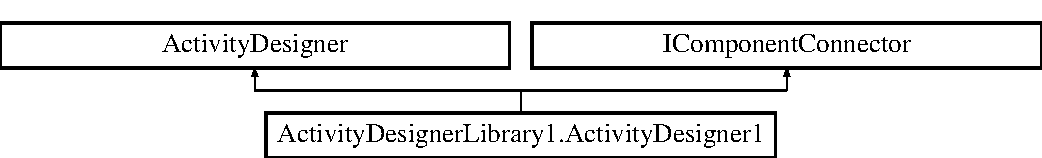
\includegraphics[height=2.000000cm]{class_activity_designer_library1_1_1_activity_designer1}
\end{center}
\end{figure}
\subsection*{Public Member Functions}
\begin{DoxyCompactItemize}
\item 
void \hyperlink{class_activity_designer_library1_1_1_activity_designer1_a1c79b52865a8360b0a02e7305d818eb2}{Initialize\+Component} ()
\begin{DoxyCompactList}\small\item\em Initialize\+Component \end{DoxyCompactList}\end{DoxyCompactItemize}


\subsection{Detailed Description}
\hyperlink{class_activity_designer_library1_1_1_activity_designer1}{Activity\+Designer1} 



\subsection{Member Function Documentation}
\index{Activity\+Designer\+Library1\+::\+Activity\+Designer1@{Activity\+Designer\+Library1\+::\+Activity\+Designer1}!Initialize\+Component@{Initialize\+Component}}
\index{Initialize\+Component@{Initialize\+Component}!Activity\+Designer\+Library1\+::\+Activity\+Designer1@{Activity\+Designer\+Library1\+::\+Activity\+Designer1}}
\subsubsection[{\texorpdfstring{Initialize\+Component()}{InitializeComponent()}}]{\setlength{\rightskip}{0pt plus 5cm}void Activity\+Designer\+Library1.\+Activity\+Designer1.\+Initialize\+Component (
\begin{DoxyParamCaption}
{}
\end{DoxyParamCaption}
)\hspace{0.3cm}{\ttfamily [inline]}}\hypertarget{class_activity_designer_library1_1_1_activity_designer1_a1c79b52865a8360b0a02e7305d818eb2}{}\label{class_activity_designer_library1_1_1_activity_designer1_a1c79b52865a8360b0a02e7305d818eb2}


Initialize\+Component 



The documentation for this class was generated from the following files\+:\begin{DoxyCompactItemize}
\item 
Activity\+Designer\+Library1/Activity\+Designer1.\+xaml.\+cs\item 
Activity\+Designer\+Library1/obj/\+Debug/Activity\+Designer1.\+g.\+i.\+cs\end{DoxyCompactItemize}

\hypertarget{class__1920_parser_1_1_group_node}{}\section{\+\_\+1920\+Parser.\+Group\+Node Class Reference}
\label{class__1920_parser_1_1_group_node}\index{\+\_\+1920\+Parser.\+Group\+Node@{\+\_\+1920\+Parser.\+Group\+Node}}


\hyperlink{class__1920_parser_1_1_group_node}{Group\+Node} represents an internal node.  




Inherits \hyperlink{class__1920_parser_1_1_abstract_node}{\+\_\+1920\+Parser.\+Abstract\+Node}.

\subsection*{Public Member Functions}
\begin{DoxyCompactItemize}
\item 
{\bfseries Group\+Node} (bool redefines, int level, string var\+Name, int repeat\+Count, int repeat\+Index, string comment)\hypertarget{class__1920_parser_1_1_group_node_a53519a72e3f5194de29b77e51f5df939}{}\label{class__1920_parser_1_1_group_node_a53519a72e3f5194de29b77e51f5df939}

\item 
override int \hyperlink{class__1920_parser_1_1_group_node_a27b61720154a26499149966cf22de811}{Assign\+Value} (string data)
\begin{DoxyCompactList}\small\item\em Assigns substrings of data to its children. The begin of a substring shifts with each assignment to a child. \end{DoxyCompactList}\item 
override string \hyperlink{class__1920_parser_1_1_group_node_a9d5c05eabdd12c9c4ca306cc369d8523}{To\+String} (int tab\+Count)
\begin{DoxyCompactList}\small\item\em Returns a string representing this \hyperlink{class__1920_parser_1_1_group_node}{Group\+Node} and its children. \end{DoxyCompactList}\item 
override \hyperlink{class__1920_parser_1_1_abstract_node}{Abstract\+Node} \hyperlink{class__1920_parser_1_1_group_node_ab01b00a2bbbef1d565e5ef3e951c4ed6}{Create\+Copy\+With\+Index} (int index)
\begin{DoxyCompactList}\small\item\em Creates a deep copy of this \hyperlink{class__1920_parser_1_1_group_node}{Group\+Node} and sets its Repeat\+Index to the value of the parameter. \end{DoxyCompactList}\item 
override void \hyperlink{class__1920_parser_1_1_group_node_a037839ecea0ec7326c6a49e0793bd6c8}{Add\+Child} (\hyperlink{class__1920_parser_1_1_abstract_node}{Abstract\+Node} child)
\begin{DoxyCompactList}\small\item\em Adds a child node. The child could be another \hyperlink{class__1920_parser_1_1_group_node}{Group\+Node}. \end{DoxyCompactList}\item 
override int \hyperlink{class__1920_parser_1_1_group_node_a314c8fb4d4f71b11916df9c822b9442d}{Get\+Hash\+Code} ()
\begin{DoxyCompactList}\small\item\em Returns the Hashcode of this class. This method is not supposed to be called directly, it was overwritten in conjunction with \hyperlink{class__1920_parser_1_1_group_node_a944b36a0063df009c7f554522f7e38fc}{Equals()}. \end{DoxyCompactList}\item 
override bool \hyperlink{class__1920_parser_1_1_group_node_a944b36a0063df009c7f554522f7e38fc}{Equals} (object obj)
\begin{DoxyCompactList}\small\item\em Compares two Group\+Nodes. Group\+Nodes are equal if all their attributes are equal and the attributes of all their children are equal. \end{DoxyCompactList}\end{DoxyCompactItemize}
\subsection*{Additional Inherited Members}


\subsection{Detailed Description}
\hyperlink{class__1920_parser_1_1_group_node}{Group\+Node} represents an internal node. 



\subsection{Member Function Documentation}
\index{\+\_\+1920\+Parser\+::\+Group\+Node@{\+\_\+1920\+Parser\+::\+Group\+Node}!Add\+Child@{Add\+Child}}
\index{Add\+Child@{Add\+Child}!\+\_\+1920\+Parser\+::\+Group\+Node@{\+\_\+1920\+Parser\+::\+Group\+Node}}
\subsubsection[{\texorpdfstring{Add\+Child(\+Abstract\+Node child)}{AddChild(AbstractNode child)}}]{\setlength{\rightskip}{0pt plus 5cm}override void \+\_\+1920\+Parser.\+Group\+Node.\+Add\+Child (
\begin{DoxyParamCaption}
\item[{{\bf Abstract\+Node}}]{child}
\end{DoxyParamCaption}
)\hspace{0.3cm}{\ttfamily [inline]}, {\ttfamily [virtual]}}\hypertarget{class__1920_parser_1_1_group_node_a037839ecea0ec7326c6a49e0793bd6c8}{}\label{class__1920_parser_1_1_group_node_a037839ecea0ec7326c6a49e0793bd6c8}


Adds a child node. The child could be another \hyperlink{class__1920_parser_1_1_group_node}{Group\+Node}. 



Implements \hyperlink{class__1920_parser_1_1_abstract_node}{\+\_\+1920\+Parser.\+Abstract\+Node}.

\index{\+\_\+1920\+Parser\+::\+Group\+Node@{\+\_\+1920\+Parser\+::\+Group\+Node}!Assign\+Value@{Assign\+Value}}
\index{Assign\+Value@{Assign\+Value}!\+\_\+1920\+Parser\+::\+Group\+Node@{\+\_\+1920\+Parser\+::\+Group\+Node}}
\subsubsection[{\texorpdfstring{Assign\+Value(string data)}{AssignValue(string data)}}]{\setlength{\rightskip}{0pt plus 5cm}override int \+\_\+1920\+Parser.\+Group\+Node.\+Assign\+Value (
\begin{DoxyParamCaption}
\item[{string}]{data}
\end{DoxyParamCaption}
)\hspace{0.3cm}{\ttfamily [inline]}, {\ttfamily [virtual]}}\hypertarget{class__1920_parser_1_1_group_node_a27b61720154a26499149966cf22de811}{}\label{class__1920_parser_1_1_group_node_a27b61720154a26499149966cf22de811}


Assigns substrings of data to its children. The begin of a substring shifts with each assignment to a child. 


\begin{DoxyParams}{Parameters}
{\em data} & \\
\hline
\end{DoxyParams}
\begin{DoxyReturn}{Returns}

\end{DoxyReturn}


Implements \hyperlink{class__1920_parser_1_1_abstract_node}{\+\_\+1920\+Parser.\+Abstract\+Node}.

\index{\+\_\+1920\+Parser\+::\+Group\+Node@{\+\_\+1920\+Parser\+::\+Group\+Node}!Create\+Copy\+With\+Index@{Create\+Copy\+With\+Index}}
\index{Create\+Copy\+With\+Index@{Create\+Copy\+With\+Index}!\+\_\+1920\+Parser\+::\+Group\+Node@{\+\_\+1920\+Parser\+::\+Group\+Node}}
\subsubsection[{\texorpdfstring{Create\+Copy\+With\+Index(int index)}{CreateCopyWithIndex(int index)}}]{\setlength{\rightskip}{0pt plus 5cm}override {\bf Abstract\+Node} \+\_\+1920\+Parser.\+Group\+Node.\+Create\+Copy\+With\+Index (
\begin{DoxyParamCaption}
\item[{int}]{index}
\end{DoxyParamCaption}
)\hspace{0.3cm}{\ttfamily [inline]}, {\ttfamily [virtual]}}\hypertarget{class__1920_parser_1_1_group_node_ab01b00a2bbbef1d565e5ef3e951c4ed6}{}\label{class__1920_parser_1_1_group_node_ab01b00a2bbbef1d565e5ef3e951c4ed6}


Creates a deep copy of this \hyperlink{class__1920_parser_1_1_group_node}{Group\+Node} and sets its Repeat\+Index to the value of the parameter. 


\begin{DoxyParams}{Parameters}
{\em index} & The index.\\
\hline
\end{DoxyParams}
\begin{DoxyReturn}{Returns}

\end{DoxyReturn}


Implements \hyperlink{class__1920_parser_1_1_abstract_node}{\+\_\+1920\+Parser.\+Abstract\+Node}.

\index{\+\_\+1920\+Parser\+::\+Group\+Node@{\+\_\+1920\+Parser\+::\+Group\+Node}!Equals@{Equals}}
\index{Equals@{Equals}!\+\_\+1920\+Parser\+::\+Group\+Node@{\+\_\+1920\+Parser\+::\+Group\+Node}}
\subsubsection[{\texorpdfstring{Equals(object obj)}{Equals(object obj)}}]{\setlength{\rightskip}{0pt plus 5cm}override bool \+\_\+1920\+Parser.\+Group\+Node.\+Equals (
\begin{DoxyParamCaption}
\item[{object}]{obj}
\end{DoxyParamCaption}
)\hspace{0.3cm}{\ttfamily [inline]}}\hypertarget{class__1920_parser_1_1_group_node_a944b36a0063df009c7f554522f7e38fc}{}\label{class__1920_parser_1_1_group_node_a944b36a0063df009c7f554522f7e38fc}


Compares two Group\+Nodes. Group\+Nodes are equal if all their attributes are equal and the attributes of all their children are equal. 

\index{\+\_\+1920\+Parser\+::\+Group\+Node@{\+\_\+1920\+Parser\+::\+Group\+Node}!Get\+Hash\+Code@{Get\+Hash\+Code}}
\index{Get\+Hash\+Code@{Get\+Hash\+Code}!\+\_\+1920\+Parser\+::\+Group\+Node@{\+\_\+1920\+Parser\+::\+Group\+Node}}
\subsubsection[{\texorpdfstring{Get\+Hash\+Code()}{GetHashCode()}}]{\setlength{\rightskip}{0pt plus 5cm}override int \+\_\+1920\+Parser.\+Group\+Node.\+Get\+Hash\+Code (
\begin{DoxyParamCaption}
{}
\end{DoxyParamCaption}
)\hspace{0.3cm}{\ttfamily [inline]}}\hypertarget{class__1920_parser_1_1_group_node_a314c8fb4d4f71b11916df9c822b9442d}{}\label{class__1920_parser_1_1_group_node_a314c8fb4d4f71b11916df9c822b9442d}


Returns the Hashcode of this class. This method is not supposed to be called directly, it was overwritten in conjunction with \hyperlink{class__1920_parser_1_1_group_node_a944b36a0063df009c7f554522f7e38fc}{Equals()}. 

\index{\+\_\+1920\+Parser\+::\+Group\+Node@{\+\_\+1920\+Parser\+::\+Group\+Node}!To\+String@{To\+String}}
\index{To\+String@{To\+String}!\+\_\+1920\+Parser\+::\+Group\+Node@{\+\_\+1920\+Parser\+::\+Group\+Node}}
\subsubsection[{\texorpdfstring{To\+String(int tab\+Count)}{ToString(int tabCount)}}]{\setlength{\rightskip}{0pt plus 5cm}override string \+\_\+1920\+Parser.\+Group\+Node.\+To\+String (
\begin{DoxyParamCaption}
\item[{int}]{tab\+Count}
\end{DoxyParamCaption}
)\hspace{0.3cm}{\ttfamily [inline]}, {\ttfamily [virtual]}}\hypertarget{class__1920_parser_1_1_group_node_a9d5c05eabdd12c9c4ca306cc369d8523}{}\label{class__1920_parser_1_1_group_node_a9d5c05eabdd12c9c4ca306cc369d8523}


Returns a string representing this \hyperlink{class__1920_parser_1_1_group_node}{Group\+Node} and its children. 


\begin{DoxyParams}{Parameters}
{\em tab\+Count} & indicates how much the string is indented. \begin{DoxyReturn}{Returns}
A System.\+String that represents this instance. 
\end{DoxyReturn}
\\
\hline
\end{DoxyParams}


Implements \hyperlink{class__1920_parser_1_1_abstract_node}{\+\_\+1920\+Parser.\+Abstract\+Node}.



The documentation for this class was generated from the following file\+:\begin{DoxyCompactItemize}
\item 
1920\+Parser/Group\+Node.\+cs\end{DoxyCompactItemize}

\hypertarget{class__1920_parser_test_1_1_group_node_test}{}\section{\+\_\+1920\+Parser\+Test.\+Group\+Node\+Test Class Reference}
\label{class__1920_parser_test_1_1_group_node_test}\index{\+\_\+1920\+Parser\+Test.\+Group\+Node\+Test@{\+\_\+1920\+Parser\+Test.\+Group\+Node\+Test}}


This is a test class for \hyperlink{class__1920_parser_test_1_1_group_node_test}{Group\+Node\+Test} and is intended to contain all \hyperlink{class__1920_parser_test_1_1_group_node_test}{Group\+Node\+Test} Unit Tests /summary$>$  


\subsection*{Public Member Functions}
\begin{DoxyCompactItemize}
\item 
void \hyperlink{class__1920_parser_test_1_1_group_node_test_a2cb1adf10d46b843dbbc1fe4691cde4a}{Group\+Nodes\+With\+Equal\+Values\+And\+Equal\+Children\+Are\+Equal\+Test} ()\hypertarget{class__1920_parser_test_1_1_group_node_test_a2cb1adf10d46b843dbbc1fe4691cde4a}{}\label{class__1920_parser_test_1_1_group_node_test_a2cb1adf10d46b843dbbc1fe4691cde4a}

\begin{DoxyCompactList}\small\item\em Group\+Nodes with equal attribute values are equal, if all their children are equal too /summary$>$ \end{DoxyCompactList}\item 
void \hyperlink{class__1920_parser_test_1_1_group_node_test_a871e698fdbcb73b2564ac6cb48ca8031}{Group\+Nodes\+With\+Equal\+Values\+And\+Different\+Children\+Are\+Not\+Equal\+Test} ()\hypertarget{class__1920_parser_test_1_1_group_node_test_a871e698fdbcb73b2564ac6cb48ca8031}{}\label{class__1920_parser_test_1_1_group_node_test_a871e698fdbcb73b2564ac6cb48ca8031}

\begin{DoxyCompactList}\small\item\em Group\+Nodes with equal attribute values are equal, if all their children are equal too /summary$>$ \end{DoxyCompactList}\item 
void \hyperlink{class__1920_parser_test_1_1_group_node_test_a9ae167ae89a66c97c605a1d99c4e9169}{Groupt\+Assign\+Value\+Test} ()\hypertarget{class__1920_parser_test_1_1_group_node_test_a9ae167ae89a66c97c605a1d99c4e9169}{}\label{class__1920_parser_test_1_1_group_node_test_a9ae167ae89a66c97c605a1d99c4e9169}

\begin{DoxyCompactList}\small\item\em A test for Assign\+Value /summary$>$ \end{DoxyCompactList}\end{DoxyCompactItemize}
\subsection*{Properties}
\begin{DoxyCompactItemize}
\item 
Test\+Context \hyperlink{class__1920_parser_test_1_1_group_node_test_abc5b4617a242e194056eaf7d5a2d28f8}{Test\+Context}\hspace{0.3cm}{\ttfamily  \mbox{[}get, set\mbox{]}}\hypertarget{class__1920_parser_test_1_1_group_node_test_abc5b4617a242e194056eaf7d5a2d28f8}{}\label{class__1920_parser_test_1_1_group_node_test_abc5b4617a242e194056eaf7d5a2d28f8}

\begin{DoxyCompactList}\small\item\em Gets or sets the test context which provides information about and functionality for the current test run. /summary$>$ \end{DoxyCompactList}\end{DoxyCompactItemize}


\subsection{Detailed Description}
This is a test class for \hyperlink{class__1920_parser_test_1_1_group_node_test}{Group\+Node\+Test} and is intended to contain all \hyperlink{class__1920_parser_test_1_1_group_node_test}{Group\+Node\+Test} Unit Tests /summary$>$ 

The documentation for this class was generated from the following file\+:\begin{DoxyCompactItemize}
\item 
1920\+Parser\+Test/Group\+Node\+Test.\+cs\end{DoxyCompactItemize}

\hypertarget{class_ranking}{}\section{Ranking Class Reference}
\label{class_ranking}\index{Ranking@{Ranking}}
\subsection*{Public Member Functions}
\begin{DoxyCompactItemize}
\item 
{\bfseries \+\_\+\+\_\+construct} (\$file, \$title, \$rank)\hypertarget{class_ranking_afe0e442564f7e3a0adc2876114529875}{}\label{class_ranking_afe0e442564f7e3a0adc2876114529875}

\item 
{\bfseries \+\_\+\+\_\+construct} (\$file, \$title, \$rank)\hypertarget{class_ranking_afe0e442564f7e3a0adc2876114529875}{}\label{class_ranking_afe0e442564f7e3a0adc2876114529875}

\item 
{\bfseries \+\_\+\+\_\+construct} (\$file, \$title, \$rank)\hypertarget{class_ranking_afe0e442564f7e3a0adc2876114529875}{}\label{class_ranking_afe0e442564f7e3a0adc2876114529875}

\item 
{\bfseries \+\_\+\+\_\+construct} (\$file, \$title, \$rank)\hypertarget{class_ranking_afe0e442564f7e3a0adc2876114529875}{}\label{class_ranking_afe0e442564f7e3a0adc2876114529875}

\end{DoxyCompactItemize}
\subsection*{Public Attributes}
\begin{DoxyCompactItemize}
\item 
{\bfseries \$filename}\hypertarget{class_ranking_a1e4984ec7e4c36e708eb28b8be2391f7}{}\label{class_ranking_a1e4984ec7e4c36e708eb28b8be2391f7}

\item 
{\bfseries \$page\+Title}\hypertarget{class_ranking_a0056f5cd56d4064ff87ac7320cfb6015}{}\label{class_ranking_a0056f5cd56d4064ff87ac7320cfb6015}

\item 
{\bfseries \$rank}\hypertarget{class_ranking_ab5257619a8e402eb95339f60aff1376c}{}\label{class_ranking_ab5257619a8e402eb95339f60aff1376c}

\end{DoxyCompactItemize}


The documentation for this class was generated from the following file\+:\begin{DoxyCompactItemize}
\item 
packages/\+E\+W\+Software.\+S\+H\+F\+B.\+2016.\+4.\+9.\+0/tools/\+Presentation\+Styles/\+Legacy\+Web/Search\+Help.\+inc.\+php\end{DoxyCompactItemize}

\hypertarget{class__1920_parser_1_1_save_schema_form}{}\section{\+\_\+1920\+Parser.\+Save\+Schema\+Form Class Reference}
\label{class__1920_parser_1_1_save_schema_form}\index{\+\_\+1920\+Parser.\+Save\+Schema\+Form@{\+\_\+1920\+Parser.\+Save\+Schema\+Form}}
Inheritance diagram for \+\_\+1920\+Parser.\+Save\+Schema\+Form\+:\begin{figure}[H]
\begin{center}
\leavevmode
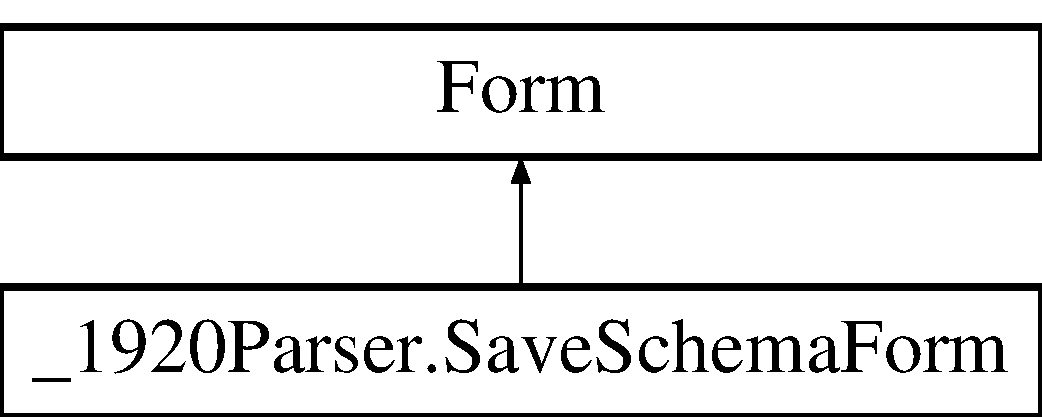
\includegraphics[height=2.000000cm]{class__1920_parser_1_1_save_schema_form}
\end{center}
\end{figure}
\subsection*{Public Member Functions}
\begin{DoxyCompactItemize}
\item 
void {\bfseries set\+Files\+Already\+Used} (I\+Enumerable$<$ string $>$ files)\hypertarget{class__1920_parser_1_1_save_schema_form_a16d5555788d91934ca0e62f9e45fd21d}{}\label{class__1920_parser_1_1_save_schema_form_a16d5555788d91934ca0e62f9e45fd21d}

\end{DoxyCompactItemize}
\subsection*{Public Attributes}
\begin{DoxyCompactItemize}
\item 
System.\+Windows.\+Forms.\+Text\+Box {\bfseries tb\+Schema\+Name}\hypertarget{class__1920_parser_1_1_save_schema_form_ae4760769155fc202f53ea12b63d14633}{}\label{class__1920_parser_1_1_save_schema_form_ae4760769155fc202f53ea12b63d14633}

\item 
System.\+Windows.\+Forms.\+Text\+Box {\bfseries tb\+Data\+Identifier}\hypertarget{class__1920_parser_1_1_save_schema_form_a6b4727fdf859c257a72b637ffae15bdc}{}\label{class__1920_parser_1_1_save_schema_form_a6b4727fdf859c257a72b637ffae15bdc}

\item 
System.\+Windows.\+Forms.\+Numeric\+Up\+Down {\bfseries nud\+Data\+Identifier\+Position}\hypertarget{class__1920_parser_1_1_save_schema_form_afb1dbb18d04daa7d93d504ebf2b28dae}{}\label{class__1920_parser_1_1_save_schema_form_afb1dbb18d04daa7d93d504ebf2b28dae}

\end{DoxyCompactItemize}
\subsection*{Protected Member Functions}
\begin{DoxyCompactItemize}
\item 
override void \hyperlink{class__1920_parser_1_1_save_schema_form_aad5b4dd643ce36c4f44b98d98b2c3a06}{Dispose} (bool disposing)
\begin{DoxyCompactList}\small\item\em Clean up any resources being used. \end{DoxyCompactList}\end{DoxyCompactItemize}
\subsection*{Properties}
\begin{DoxyCompactItemize}
\item 
string {\bfseries Data}\hspace{0.3cm}{\ttfamily  \mbox{[}get, set\mbox{]}}\hypertarget{class__1920_parser_1_1_save_schema_form_a81a2de8249e6b56fbf8f3869f6664f1a}{}\label{class__1920_parser_1_1_save_schema_form_a81a2de8249e6b56fbf8f3869f6664f1a}

\item 
string {\bfseries Name1}\hspace{0.3cm}{\ttfamily  \mbox{[}get, set\mbox{]}}\hypertarget{class__1920_parser_1_1_save_schema_form_a8591699ca2aa3851d5fd7a6a619e7215}{}\label{class__1920_parser_1_1_save_schema_form_a8591699ca2aa3851d5fd7a6a619e7215}

\item 
int {\bfseries Position}\hspace{0.3cm}{\ttfamily  \mbox{[}get, set\mbox{]}}\hypertarget{class__1920_parser_1_1_save_schema_form_a52d14651e4fbab20200e0c6e826b48fe}{}\label{class__1920_parser_1_1_save_schema_form_a52d14651e4fbab20200e0c6e826b48fe}

\item 
string {\bfseries Value}\hspace{0.3cm}{\ttfamily  \mbox{[}get, set\mbox{]}}\hypertarget{class__1920_parser_1_1_save_schema_form_a68c8f0527dcaa8c7075eab2e0a8af8e1}{}\label{class__1920_parser_1_1_save_schema_form_a68c8f0527dcaa8c7075eab2e0a8af8e1}

\end{DoxyCompactItemize}


\subsection{Member Function Documentation}
\index{\+\_\+1920\+Parser\+::\+Save\+Schema\+Form@{\+\_\+1920\+Parser\+::\+Save\+Schema\+Form}!Dispose@{Dispose}}
\index{Dispose@{Dispose}!\+\_\+1920\+Parser\+::\+Save\+Schema\+Form@{\+\_\+1920\+Parser\+::\+Save\+Schema\+Form}}
\subsubsection[{\texorpdfstring{Dispose(bool disposing)}{Dispose(bool disposing)}}]{\setlength{\rightskip}{0pt plus 5cm}override void \+\_\+1920\+Parser.\+Save\+Schema\+Form.\+Dispose (
\begin{DoxyParamCaption}
\item[{bool}]{disposing}
\end{DoxyParamCaption}
)\hspace{0.3cm}{\ttfamily [inline]}, {\ttfamily [protected]}}\hypertarget{class__1920_parser_1_1_save_schema_form_aad5b4dd643ce36c4f44b98d98b2c3a06}{}\label{class__1920_parser_1_1_save_schema_form_aad5b4dd643ce36c4f44b98d98b2c3a06}


Clean up any resources being used. 


\begin{DoxyParams}{Parameters}
{\em disposing} & true if managed resources should be disposed; otherwise, false.\\
\hline
\end{DoxyParams}


The documentation for this class was generated from the following files\+:\begin{DoxyCompactItemize}
\item 
1920\+Parser/Save\+Schema\+Form.\+cs\item 
1920\+Parser/Save\+Schema\+Form.\+Designer.\+cs\end{DoxyCompactItemize}

\hypertarget{class__1920_parser_1_1_schema}{}\section{\+\_\+1920\+Parser.\+Schema Class Reference}
\label{class__1920_parser_1_1_schema}\index{\+\_\+1920\+Parser.\+Schema@{\+\_\+1920\+Parser.\+Schema}}
\subsection*{Public Member Functions}
\begin{DoxyCompactItemize}
\item 
\hyperlink{class__1920_parser_1_1_abstract_node}{Abstract\+Node} {\bfseries Parse\+Line} (string line)\hypertarget{class__1920_parser_1_1_schema_a7593a133f248c1ad6599fc6e706b3fb8}{}\label{class__1920_parser_1_1_schema_a7593a133f248c1ad6599fc6e706b3fb8}

\item 
\hyperlink{class__1920_parser_1_1_group_node}{Group\+Node} {\bfseries Parse} ()\hypertarget{class__1920_parser_1_1_schema_a970c7c326e6f505c5798392da0fa0385}{}\label{class__1920_parser_1_1_schema_a970c7c326e6f505c5798392da0fa0385}

\end{DoxyCompactItemize}


The documentation for this class was generated from the following file\+:\begin{DoxyCompactItemize}
\item 
1920\+Parser/Schema.\+cs\end{DoxyCompactItemize}

\hypertarget{classschemas}{}\section{schemas Class Reference}
\label{classschemas}\index{schemas@{schemas}}


 


\subsection*{Properties}
\begin{DoxyCompactItemize}
\item 
\hyperlink{classschemas_schema}{schemas\+Schema}\mbox{[}$\,$\mbox{]} \hyperlink{classschemas_adf132f5b1f6ac5984256a262fac2bb1b}{schema}\hspace{0.3cm}{\ttfamily  \mbox{[}get, set\mbox{]}}
\end{DoxyCompactItemize}


\subsection{Detailed Description}


\subsection{Property Documentation}
\index{schemas@{schemas}!schema@{schema}}
\index{schema@{schema}!schemas@{schemas}}
\subsubsection[{\texorpdfstring{schema}{schema}}]{\setlength{\rightskip}{0pt plus 5cm}{\bf schemas\+Schema} \mbox{[}$\,$\mbox{]} schemas.\+schema\hspace{0.3cm}{\ttfamily [get]}, {\ttfamily [set]}}\hypertarget{classschemas_adf132f5b1f6ac5984256a262fac2bb1b}{}\label{classschemas_adf132f5b1f6ac5984256a262fac2bb1b}






The documentation for this class was generated from the following file\+:\begin{DoxyCompactItemize}
\item 
\hyperlink{schemas_8cs}{schemas.\+cs}\end{DoxyCompactItemize}

\hypertarget{classschemas_schema}{}\section{schemas\+Schema Class Reference}
\label{classschemas_schema}\index{schemas\+Schema@{schemas\+Schema}}


 


\subsection*{Properties}
\begin{DoxyCompactItemize}
\item 
string \hyperlink{classschemas_schema_ade6edd95fc90d8c67e0c0bfe34388a79}{name}\hspace{0.3cm}{\ttfamily  \mbox{[}get, set\mbox{]}}\hypertarget{classschemas_schema_ade6edd95fc90d8c67e0c0bfe34388a79}{}\label{classschemas_schema_ade6edd95fc90d8c67e0c0bfe34388a79}

\item 
\hyperlink{classschemas_schema_identifier}{schemas\+Schema\+Identifier}\mbox{[}$\,$\mbox{]} \hyperlink{classschemas_schema_aa0f4c1fca6a4bc1a6e01d0f545a4a241}{identifiers}\hspace{0.3cm}{\ttfamily  \mbox{[}get, set\mbox{]}}\hypertarget{classschemas_schema_aa0f4c1fca6a4bc1a6e01d0f545a4a241}{}\label{classschemas_schema_aa0f4c1fca6a4bc1a6e01d0f545a4a241}

\end{DoxyCompactItemize}


\subsection{Detailed Description}


The documentation for this class was generated from the following file\+:\begin{DoxyCompactItemize}
\item 
1920\+Parser/schemas.\+cs\end{DoxyCompactItemize}

\hypertarget{classschemas_schema_identifier}{}\section{schemas\+Schema\+Identifier Class Reference}
\label{classschemas_schema_identifier}\index{schemas\+Schema\+Identifier@{schemas\+Schema\+Identifier}}


 


\subsection*{Properties}
\begin{DoxyCompactItemize}
\item 
string \hyperlink{classschemas_schema_identifier_a0dcd51bb1fb87d49765cf031b4425a46}{value}\hspace{0.3cm}{\ttfamily  \mbox{[}get, set\mbox{]}}
\item 
int \hyperlink{classschemas_schema_identifier_a050bed554a3f4564b1e029d95d020905}{start}\hspace{0.3cm}{\ttfamily  \mbox{[}get, set\mbox{]}}
\end{DoxyCompactItemize}


\subsection{Detailed Description}


\subsection{Property Documentation}
\index{schemas\+Schema\+Identifier@{schemas\+Schema\+Identifier}!start@{start}}
\index{start@{start}!schemas\+Schema\+Identifier@{schemas\+Schema\+Identifier}}
\subsubsection[{\texorpdfstring{start}{start}}]{\setlength{\rightskip}{0pt plus 5cm}int schemas\+Schema\+Identifier.\+start\hspace{0.3cm}{\ttfamily [get]}, {\ttfamily [set]}}\hypertarget{classschemas_schema_identifier_a050bed554a3f4564b1e029d95d020905}{}\label{classschemas_schema_identifier_a050bed554a3f4564b1e029d95d020905}




\index{schemas\+Schema\+Identifier@{schemas\+Schema\+Identifier}!value@{value}}
\index{value@{value}!schemas\+Schema\+Identifier@{schemas\+Schema\+Identifier}}
\subsubsection[{\texorpdfstring{value}{value}}]{\setlength{\rightskip}{0pt plus 5cm}string schemas\+Schema\+Identifier.\+value\hspace{0.3cm}{\ttfamily [get]}, {\ttfamily [set]}}\hypertarget{classschemas_schema_identifier_a0dcd51bb1fb87d49765cf031b4425a46}{}\label{classschemas_schema_identifier_a0dcd51bb1fb87d49765cf031b4425a46}






The documentation for this class was generated from the following file\+:\begin{DoxyCompactItemize}
\item 
\hyperlink{schemas_8cs}{schemas.\+cs}\end{DoxyCompactItemize}

\hypertarget{class__1920_parser_test_1_1_schema_test}{}\section{\+\_\+1920\+Parser\+Test.\+Schema\+Test Class Reference}
\label{class__1920_parser_test_1_1_schema_test}\index{\+\_\+1920\+Parser\+Test.\+Schema\+Test@{\+\_\+1920\+Parser\+Test.\+Schema\+Test}}


This is a test class for \hyperlink{class__1920_parser_test_1_1_schema_test}{Schema\+Test} and is intended to contain all \hyperlink{class__1920_parser_test_1_1_schema_test}{Schema\+Test} Unit Tests /summary$>$  


\subsection*{Public Member Functions}
\begin{DoxyCompactItemize}
\item 
void \hyperlink{class__1920_parser_test_1_1_schema_test_a942c4483675402b61174b44993515deb}{Schema\+Constructor\+Test} ()\hypertarget{class__1920_parser_test_1_1_schema_test_a942c4483675402b61174b44993515deb}{}\label{class__1920_parser_test_1_1_schema_test_a942c4483675402b61174b44993515deb}

\begin{DoxyCompactList}\small\item\em A test for Parser Constructor /summary$>$ \end{DoxyCompactList}\item 
void \hyperlink{class__1920_parser_test_1_1_schema_test_a54f701db5ae5b1f9848698556895935b}{parse\+Test1} ()\hypertarget{class__1920_parser_test_1_1_schema_test_a54f701db5ae5b1f9848698556895935b}{}\label{class__1920_parser_test_1_1_schema_test_a54f701db5ae5b1f9848698556895935b}

\begin{DoxyCompactList}\small\item\em Just a Group\+Node /summary$>$ \end{DoxyCompactList}\item 
void \hyperlink{class__1920_parser_test_1_1_schema_test_a80f5e1451406ec6e2fdbb5ed1b0c1374}{parse\+Test2} ()\hypertarget{class__1920_parser_test_1_1_schema_test_a80f5e1451406ec6e2fdbb5ed1b0c1374}{}\label{class__1920_parser_test_1_1_schema_test_a80f5e1451406ec6e2fdbb5ed1b0c1374}

\begin{DoxyCompactList}\small\item\em Just a Value\+Node /summary$>$ \end{DoxyCompactList}\item 
void \hyperlink{class__1920_parser_test_1_1_schema_test_a0c608e8ac7f4ebf18f327678e18d8a76}{parse\+Test3} ()\hypertarget{class__1920_parser_test_1_1_schema_test_a0c608e8ac7f4ebf18f327678e18d8a76}{}\label{class__1920_parser_test_1_1_schema_test_a0c608e8ac7f4ebf18f327678e18d8a76}

\begin{DoxyCompactList}\small\item\em Group\+Node with a child /summary$>$ \end{DoxyCompactList}\item 
void \hyperlink{class__1920_parser_test_1_1_schema_test_a81271f1b42fe9ea099abc8dad2a5a693}{parse\+Test4} ()\hypertarget{class__1920_parser_test_1_1_schema_test_a81271f1b42fe9ea099abc8dad2a5a693}{}\label{class__1920_parser_test_1_1_schema_test_a81271f1b42fe9ea099abc8dad2a5a693}

\begin{DoxyCompactList}\small\item\em Repeating Group\+Node /summary$>$ \end{DoxyCompactList}\item 
void \hyperlink{class__1920_parser_test_1_1_schema_test_ad23649d4c663d2e3dcb89248b7c020d6}{parse\+Test5} ()\hypertarget{class__1920_parser_test_1_1_schema_test_ad23649d4c663d2e3dcb89248b7c020d6}{}\label{class__1920_parser_test_1_1_schema_test_ad23649d4c663d2e3dcb89248b7c020d6}

\begin{DoxyCompactList}\small\item\em A test for parse /summary$>$ \end{DoxyCompactList}\item 
void \hyperlink{class__1920_parser_test_1_1_schema_test_a2b1ef3314565101371fcb29b22708c5e}{parse\+Test6} ()\hypertarget{class__1920_parser_test_1_1_schema_test_a2b1ef3314565101371fcb29b22708c5e}{}\label{class__1920_parser_test_1_1_schema_test_a2b1ef3314565101371fcb29b22708c5e}

\begin{DoxyCompactList}\small\item\em A test for parse /summary$>$ \end{DoxyCompactList}\end{DoxyCompactItemize}
\subsection*{Properties}
\begin{DoxyCompactItemize}
\item 
Test\+Context \hyperlink{class__1920_parser_test_1_1_schema_test_a2f92a3308526a2f070a7dd74dc2433e6}{Test\+Context}\hspace{0.3cm}{\ttfamily  \mbox{[}get, set\mbox{]}}\hypertarget{class__1920_parser_test_1_1_schema_test_a2f92a3308526a2f070a7dd74dc2433e6}{}\label{class__1920_parser_test_1_1_schema_test_a2f92a3308526a2f070a7dd74dc2433e6}

\begin{DoxyCompactList}\small\item\em Gets or sets the test context which provides information about and functionality for the current test run. /summary$>$ \end{DoxyCompactList}\end{DoxyCompactItemize}


\subsection{Detailed Description}
This is a test class for \hyperlink{class__1920_parser_test_1_1_schema_test}{Schema\+Test} and is intended to contain all \hyperlink{class__1920_parser_test_1_1_schema_test}{Schema\+Test} Unit Tests /summary$>$ 

The documentation for this class was generated from the following file\+:\begin{DoxyCompactItemize}
\item 
1920\+Parser\+Test/Schema\+Test.\+cs\end{DoxyCompactItemize}

\hypertarget{class__1920_parser_1_1_value_node}{}\section{\+\_\+1920\+Parser.\+Value\+Node Class Reference}
\label{class__1920_parser_1_1_value_node}\index{\+\_\+1920\+Parser.\+Value\+Node@{\+\_\+1920\+Parser.\+Value\+Node}}
Inheritance diagram for \+\_\+1920\+Parser.\+Value\+Node\+:\begin{figure}[H]
\begin{center}
\leavevmode
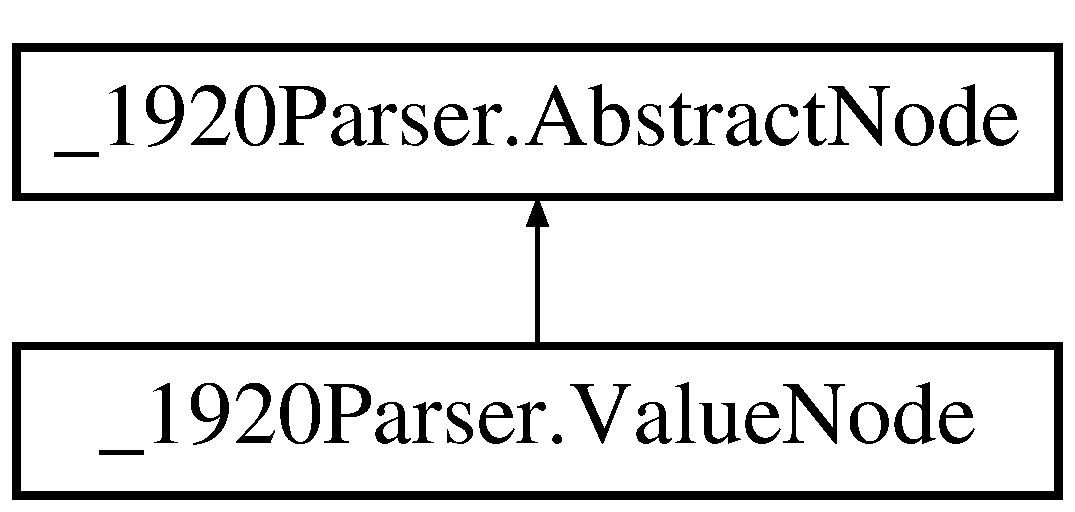
\includegraphics[height=2.000000cm]{class__1920_parser_1_1_value_node}
\end{center}
\end{figure}
\subsection*{Public Member Functions}
\begin{DoxyCompactItemize}
\item 
\hyperlink{class__1920_parser_1_1_value_node_a5070c8591d364b184fb2f7a83098d1df}{Value\+Node} (bool redefines, int level, string var\+Name, string type, int length, int repeat\+Count, int repeat\+Index, string comment)
\item 
override \hyperlink{class__1920_parser_1_1_abstract_node}{Abstract\+Node} \hyperlink{class__1920_parser_1_1_value_node_a9419a8beace8e6eda482fc3a403daf4b}{Create\+Copy\+With\+Index} (int index)
\item 
override int \hyperlink{class__1920_parser_1_1_value_node_a21bed203f8124c630e8b804ebcd7b728}{Assign\+Value} (string data)
\item 
override string \hyperlink{class__1920_parser_1_1_value_node_ae2b512cbab33936e1b02d7a7acf3b4bd}{To\+String} (int tab\+Count)
\item 
override void \hyperlink{class__1920_parser_1_1_value_node_a035c2fb0a7af286a4718e7215b2925a1}{Add\+Child} (\hyperlink{class__1920_parser_1_1_abstract_node}{Abstract\+Node} child)
\item 
override int \hyperlink{class__1920_parser_1_1_value_node_a77ab8503cab6fa67bc948c6ac7bbff09}{Get\+Hash\+Code} ()
\item 
override bool \hyperlink{class__1920_parser_1_1_value_node_a748e3fdade8e115cc73babbe19646351}{Equals} (object obj)
\end{DoxyCompactItemize}
\subsection*{Properties}
\begin{DoxyCompactItemize}
\item 
string \hyperlink{class__1920_parser_1_1_value_node_af246d6039acc23ab38b0a1b9ed741465}{Type}\hspace{0.3cm}{\ttfamily  \mbox{[}get\mbox{]}}
\item 
int \hyperlink{class__1920_parser_1_1_value_node_a373a059abbf96d88126a677665d20d9e}{Length}\hspace{0.3cm}{\ttfamily  \mbox{[}get\mbox{]}}
\item 
string \hyperlink{class__1920_parser_1_1_value_node_a56cb68d4bb4856747b88651e874d1dcd}{Value}\hspace{0.3cm}{\ttfamily  \mbox{[}get\mbox{]}}
\end{DoxyCompactItemize}


\subsection{Constructor \& Destructor Documentation}
\index{\+\_\+1920\+Parser\+::\+Value\+Node@{\+\_\+1920\+Parser\+::\+Value\+Node}!Value\+Node@{Value\+Node}}
\index{Value\+Node@{Value\+Node}!\+\_\+1920\+Parser\+::\+Value\+Node@{\+\_\+1920\+Parser\+::\+Value\+Node}}
\subsubsection[{\texorpdfstring{Value\+Node(bool redefines, int level, string var\+Name, string type, int length, int repeat\+Count, int repeat\+Index, string comment)}{ValueNode(bool redefines, int level, string varName, string type, int length, int repeatCount, int repeatIndex, string comment)}}]{\setlength{\rightskip}{0pt plus 5cm}\+\_\+1920\+Parser.\+Value\+Node.\+Value\+Node (
\begin{DoxyParamCaption}
\item[{bool}]{redefines, }
\item[{int}]{level, }
\item[{string}]{var\+Name, }
\item[{string}]{type, }
\item[{int}]{length, }
\item[{int}]{repeat\+Count, }
\item[{int}]{repeat\+Index, }
\item[{string}]{comment}
\end{DoxyParamCaption}
)}\hypertarget{class__1920_parser_1_1_value_node_a5070c8591d364b184fb2f7a83098d1df}{}\label{class__1920_parser_1_1_value_node_a5070c8591d364b184fb2f7a83098d1df}


\subsection{Member Function Documentation}
\index{\+\_\+1920\+Parser\+::\+Value\+Node@{\+\_\+1920\+Parser\+::\+Value\+Node}!Add\+Child@{Add\+Child}}
\index{Add\+Child@{Add\+Child}!\+\_\+1920\+Parser\+::\+Value\+Node@{\+\_\+1920\+Parser\+::\+Value\+Node}}
\subsubsection[{\texorpdfstring{Add\+Child(\+Abstract\+Node child)}{AddChild(AbstractNode child)}}]{\setlength{\rightskip}{0pt plus 5cm}override void \+\_\+1920\+Parser.\+Value\+Node.\+Add\+Child (
\begin{DoxyParamCaption}
\item[{{\bf Abstract\+Node}}]{child}
\end{DoxyParamCaption}
)\hspace{0.3cm}{\ttfamily [virtual]}}\hypertarget{class__1920_parser_1_1_value_node_a035c2fb0a7af286a4718e7215b2925a1}{}\label{class__1920_parser_1_1_value_node_a035c2fb0a7af286a4718e7215b2925a1}


Implements \hyperlink{class__1920_parser_1_1_abstract_node_af6241531937bb83d55aea81268b97f0b}{\+\_\+1920\+Parser.\+Abstract\+Node}.

\index{\+\_\+1920\+Parser\+::\+Value\+Node@{\+\_\+1920\+Parser\+::\+Value\+Node}!Assign\+Value@{Assign\+Value}}
\index{Assign\+Value@{Assign\+Value}!\+\_\+1920\+Parser\+::\+Value\+Node@{\+\_\+1920\+Parser\+::\+Value\+Node}}
\subsubsection[{\texorpdfstring{Assign\+Value(string data)}{AssignValue(string data)}}]{\setlength{\rightskip}{0pt plus 5cm}override int \+\_\+1920\+Parser.\+Value\+Node.\+Assign\+Value (
\begin{DoxyParamCaption}
\item[{string}]{data}
\end{DoxyParamCaption}
)\hspace{0.3cm}{\ttfamily [virtual]}}\hypertarget{class__1920_parser_1_1_value_node_a21bed203f8124c630e8b804ebcd7b728}{}\label{class__1920_parser_1_1_value_node_a21bed203f8124c630e8b804ebcd7b728}


Implements \hyperlink{class__1920_parser_1_1_abstract_node_a457498d3ec29d4c2af707aad2cf3bfc9}{\+\_\+1920\+Parser.\+Abstract\+Node}.

\index{\+\_\+1920\+Parser\+::\+Value\+Node@{\+\_\+1920\+Parser\+::\+Value\+Node}!Create\+Copy\+With\+Index@{Create\+Copy\+With\+Index}}
\index{Create\+Copy\+With\+Index@{Create\+Copy\+With\+Index}!\+\_\+1920\+Parser\+::\+Value\+Node@{\+\_\+1920\+Parser\+::\+Value\+Node}}
\subsubsection[{\texorpdfstring{Create\+Copy\+With\+Index(int index)}{CreateCopyWithIndex(int index)}}]{\setlength{\rightskip}{0pt plus 5cm}override {\bf Abstract\+Node} \+\_\+1920\+Parser.\+Value\+Node.\+Create\+Copy\+With\+Index (
\begin{DoxyParamCaption}
\item[{int}]{index}
\end{DoxyParamCaption}
)\hspace{0.3cm}{\ttfamily [virtual]}}\hypertarget{class__1920_parser_1_1_value_node_a9419a8beace8e6eda482fc3a403daf4b}{}\label{class__1920_parser_1_1_value_node_a9419a8beace8e6eda482fc3a403daf4b}


Implements \hyperlink{class__1920_parser_1_1_abstract_node_a636ae975a7e037fb31c4d4341e222c1b}{\+\_\+1920\+Parser.\+Abstract\+Node}.

\index{\+\_\+1920\+Parser\+::\+Value\+Node@{\+\_\+1920\+Parser\+::\+Value\+Node}!Equals@{Equals}}
\index{Equals@{Equals}!\+\_\+1920\+Parser\+::\+Value\+Node@{\+\_\+1920\+Parser\+::\+Value\+Node}}
\subsubsection[{\texorpdfstring{Equals(object obj)}{Equals(object obj)}}]{\setlength{\rightskip}{0pt plus 5cm}override bool \+\_\+1920\+Parser.\+Value\+Node.\+Equals (
\begin{DoxyParamCaption}
\item[{object}]{obj}
\end{DoxyParamCaption}
)}\hypertarget{class__1920_parser_1_1_value_node_a748e3fdade8e115cc73babbe19646351}{}\label{class__1920_parser_1_1_value_node_a748e3fdade8e115cc73babbe19646351}
\index{\+\_\+1920\+Parser\+::\+Value\+Node@{\+\_\+1920\+Parser\+::\+Value\+Node}!Get\+Hash\+Code@{Get\+Hash\+Code}}
\index{Get\+Hash\+Code@{Get\+Hash\+Code}!\+\_\+1920\+Parser\+::\+Value\+Node@{\+\_\+1920\+Parser\+::\+Value\+Node}}
\subsubsection[{\texorpdfstring{Get\+Hash\+Code()}{GetHashCode()}}]{\setlength{\rightskip}{0pt plus 5cm}override int \+\_\+1920\+Parser.\+Value\+Node.\+Get\+Hash\+Code (
\begin{DoxyParamCaption}
{}
\end{DoxyParamCaption}
)}\hypertarget{class__1920_parser_1_1_value_node_a77ab8503cab6fa67bc948c6ac7bbff09}{}\label{class__1920_parser_1_1_value_node_a77ab8503cab6fa67bc948c6ac7bbff09}
\index{\+\_\+1920\+Parser\+::\+Value\+Node@{\+\_\+1920\+Parser\+::\+Value\+Node}!To\+String@{To\+String}}
\index{To\+String@{To\+String}!\+\_\+1920\+Parser\+::\+Value\+Node@{\+\_\+1920\+Parser\+::\+Value\+Node}}
\subsubsection[{\texorpdfstring{To\+String(int tab\+Count)}{ToString(int tabCount)}}]{\setlength{\rightskip}{0pt plus 5cm}override string \+\_\+1920\+Parser.\+Value\+Node.\+To\+String (
\begin{DoxyParamCaption}
\item[{int}]{tab\+Count}
\end{DoxyParamCaption}
)\hspace{0.3cm}{\ttfamily [virtual]}}\hypertarget{class__1920_parser_1_1_value_node_ae2b512cbab33936e1b02d7a7acf3b4bd}{}\label{class__1920_parser_1_1_value_node_ae2b512cbab33936e1b02d7a7acf3b4bd}


Implements \hyperlink{class__1920_parser_1_1_abstract_node_ae41877e0bad1b9ed1e4b5ae8c01bca60}{\+\_\+1920\+Parser.\+Abstract\+Node}.



\subsection{Property Documentation}
\index{\+\_\+1920\+Parser\+::\+Value\+Node@{\+\_\+1920\+Parser\+::\+Value\+Node}!Length@{Length}}
\index{Length@{Length}!\+\_\+1920\+Parser\+::\+Value\+Node@{\+\_\+1920\+Parser\+::\+Value\+Node}}
\subsubsection[{\texorpdfstring{Length}{Length}}]{\setlength{\rightskip}{0pt plus 5cm}int \+\_\+1920\+Parser.\+Value\+Node.\+Length\hspace{0.3cm}{\ttfamily [get]}, {\ttfamily [protected]}}\hypertarget{class__1920_parser_1_1_value_node_a373a059abbf96d88126a677665d20d9e}{}\label{class__1920_parser_1_1_value_node_a373a059abbf96d88126a677665d20d9e}
\index{\+\_\+1920\+Parser\+::\+Value\+Node@{\+\_\+1920\+Parser\+::\+Value\+Node}!Type@{Type}}
\index{Type@{Type}!\+\_\+1920\+Parser\+::\+Value\+Node@{\+\_\+1920\+Parser\+::\+Value\+Node}}
\subsubsection[{\texorpdfstring{Type}{Type}}]{\setlength{\rightskip}{0pt plus 5cm}string \+\_\+1920\+Parser.\+Value\+Node.\+Type\hspace{0.3cm}{\ttfamily [get]}, {\ttfamily [protected]}}\hypertarget{class__1920_parser_1_1_value_node_af246d6039acc23ab38b0a1b9ed741465}{}\label{class__1920_parser_1_1_value_node_af246d6039acc23ab38b0a1b9ed741465}
\index{\+\_\+1920\+Parser\+::\+Value\+Node@{\+\_\+1920\+Parser\+::\+Value\+Node}!Value@{Value}}
\index{Value@{Value}!\+\_\+1920\+Parser\+::\+Value\+Node@{\+\_\+1920\+Parser\+::\+Value\+Node}}
\subsubsection[{\texorpdfstring{Value}{Value}}]{\setlength{\rightskip}{0pt plus 5cm}string \+\_\+1920\+Parser.\+Value\+Node.\+Value\hspace{0.3cm}{\ttfamily [get]}, {\ttfamily [protected]}}\hypertarget{class__1920_parser_1_1_value_node_a56cb68d4bb4856747b88651e874d1dcd}{}\label{class__1920_parser_1_1_value_node_a56cb68d4bb4856747b88651e874d1dcd}


The documentation for this class was generated from the following file\+:\begin{DoxyCompactItemize}
\item 
\hyperlink{_value_node_8cs}{Value\+Node.\+cs}\end{DoxyCompactItemize}

\hypertarget{class__1920_parser_test_1_1_value_node_test}{}\section{\+\_\+1920\+Parser\+Test.\+Value\+Node\+Test Class Reference}
\label{class__1920_parser_test_1_1_value_node_test}\index{\+\_\+1920\+Parser\+Test.\+Value\+Node\+Test@{\+\_\+1920\+Parser\+Test.\+Value\+Node\+Test}}


This is a test class for \hyperlink{class__1920_parser_test_1_1_value_node_test}{Value\+Node\+Test} and is intended to contain all \hyperlink{class__1920_parser_test_1_1_value_node_test}{Value\+Node\+Test} Unit Tests /summary$>$  


\subsection*{Public Member Functions}
\begin{DoxyCompactItemize}
\item 
void \hyperlink{class__1920_parser_test_1_1_value_node_test_a3241f6e4d162f00c3a4dccb1290efffc}{Value\+Nodes\+With\+Sam\+Aeattribute\+Values\+Are\+Equal} ()\hypertarget{class__1920_parser_test_1_1_value_node_test_a3241f6e4d162f00c3a4dccb1290efffc}{}\label{class__1920_parser_test_1_1_value_node_test_a3241f6e4d162f00c3a4dccb1290efffc}

\begin{DoxyCompactList}\small\item\em Value\+Nodes with equal attribute values are equal /summary$>$ \end{DoxyCompactList}\item 
void \hyperlink{class__1920_parser_test_1_1_value_node_test_af7c5889f21a4113c8103c3acdfef291b}{Value\+Nodes\+With\+Different\+Attribute\+Values\+Are\+Not\+Equal} ()\hypertarget{class__1920_parser_test_1_1_value_node_test_af7c5889f21a4113c8103c3acdfef291b}{}\label{class__1920_parser_test_1_1_value_node_test_af7c5889f21a4113c8103c3acdfef291b}

\begin{DoxyCompactList}\small\item\em Value\+Nodes with 1 or more different attribute values are not equal /summary$>$ \end{DoxyCompactList}\item 
void \hyperlink{class__1920_parser_test_1_1_value_node_test_a0c4864257368d8dff33254966a7a98ef}{To\+String\+Test} ()\hypertarget{class__1920_parser_test_1_1_value_node_test_a0c4864257368d8dff33254966a7a98ef}{}\label{class__1920_parser_test_1_1_value_node_test_a0c4864257368d8dff33254966a7a98ef}

\begin{DoxyCompactList}\small\item\em A test for To\+String /summary$>$ \end{DoxyCompactList}\item 
void \hyperlink{class__1920_parser_test_1_1_value_node_test_a99c88a4e50cdb9851954619658fe6211}{To\+String\+Test1} ()\hypertarget{class__1920_parser_test_1_1_value_node_test_a99c88a4e50cdb9851954619658fe6211}{}\label{class__1920_parser_test_1_1_value_node_test_a99c88a4e50cdb9851954619658fe6211}

\begin{DoxyCompactList}\small\item\em A test for To\+String /summary$>$ \end{DoxyCompactList}\end{DoxyCompactItemize}


\subsection{Detailed Description}
This is a test class for \hyperlink{class__1920_parser_test_1_1_value_node_test}{Value\+Node\+Test} and is intended to contain all \hyperlink{class__1920_parser_test_1_1_value_node_test}{Value\+Node\+Test} Unit Tests /summary$>$ 

The documentation for this class was generated from the following file\+:\begin{DoxyCompactItemize}
\item 
1920\+Parser\+Test/Value\+Node\+Test.\+cs\end{DoxyCompactItemize}

%--- End generated contents ---

% Index
\backmatter
\newpage
\phantomsection
\clearemptydoublepage
\addcontentsline{toc}{chapter}{Index}
\printindex

\end{document}
